\chapter{Pāli Lessons}

These lessons can be included during a Vinaya study period. The material
focues on the language forms used in the Pāṭimokkha, and introduces Pāli
readings from the rules and examples from the daily chants which
bhikkhus have already memorized.

One lesson may take more than one session to study with a group. Someone
familiar with the language may explain the grammar points, while the
others may take turns in solving the exercises.

\href{./includes/docs/pali-lessons.pdf}{pali-lessons.pdf}

\href{./includes/docs/pali-lessons-answerkey.pdf}{pali-lessons-answerkey.pdf}

\href{./includes/docs/pali-lessons.pdf}{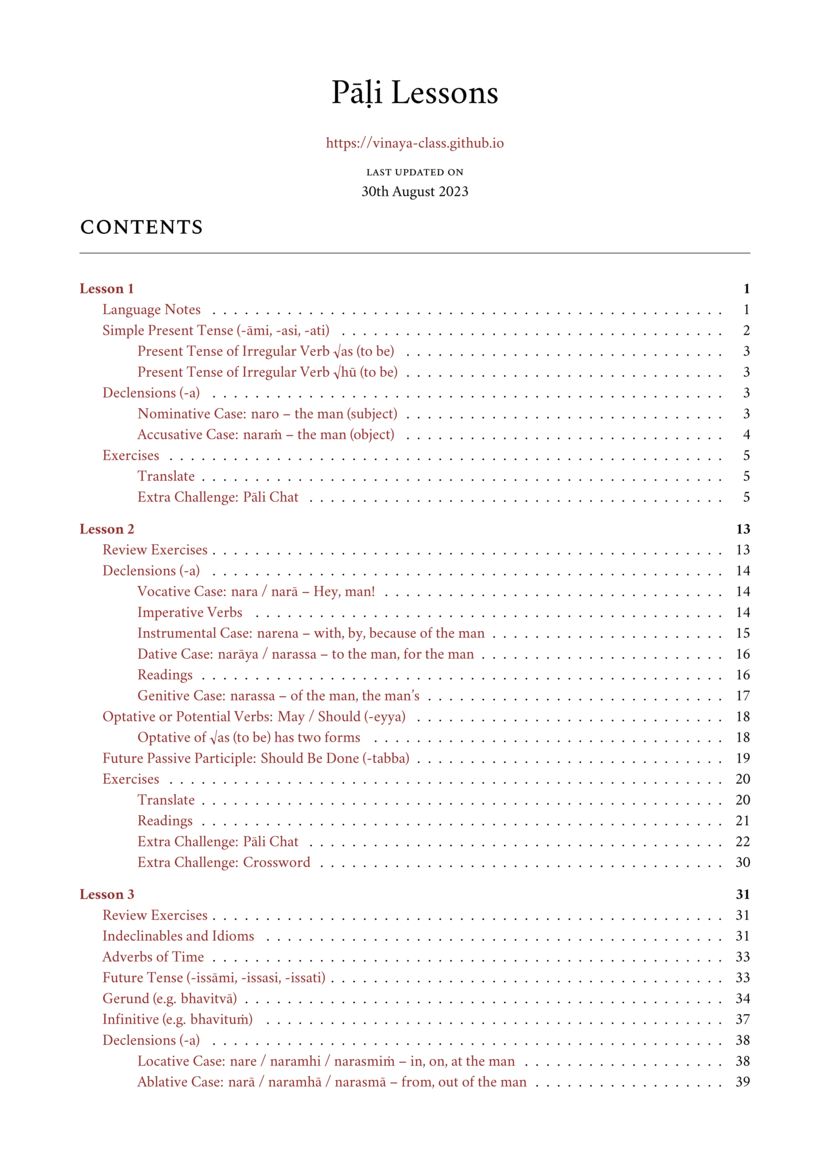
\includegraphics{./includes/docs/pali-lessons-thumb.png}}

A memory card deck for the \href{https://apps.ankiweb.net/}{Anki
application} is included below to help memorizing the vocabulary and
sentences using the \href{https://gwern.net/spaced-repetition}{Spaced
Repetition} method.

\href{./includes/docs/pali-lessons.apkg}{pali-lessons.apkg}

When you import it into Anki for the first time, it will create the
relevant card decks.

The above file gets updated as the lesson content develops. When you
import it again, Anki creates duplicate cards, which can be removed with
these steps:

\begin{enumerate}
\def\labelenumi{\arabic{enumi}.}
\tightlist
\item
  After importing, select Browse \textgreater{} Find Duplicates
  \textgreater{} `Front' field can tag the duplicates.
\item
  Search for: \texttt{tag:duplicate\ is:new}
\item
  Which can be all deleted.
\item
  Select the tag `duplicate' from the sidebar and delete the tag itself,
  which will remove it from the existing notes.
\end{enumerate}

